% Motivation, main objectives, tools, deliverables, bi-weekly timeline

\section*{Some Background and Motivation}

Sea shells have interesting patterns which  appear to be readily described by mathematics and computation. Work has already been done to describe aspects of sea shells, from the spiral shape to the color patterns to the protrusions found on the exterior \cite{Galbraith00modelingmurex}\cite{abss}\cite{VANDERHELM1998505}. Recently some work has also gone into the 3D printing of sea shell model \cite{3dprinting-seashells}\cite{bachman-3dprinting}.

The motivation of this project will be to extend the methods of generating the exterior protrusions to be able to mimic a wider variety of shells. Prusinkiewicz and Fowler have modeled periodic ridge and bump patterns and they have also combined multiple generating curves to imitate more intricate shells \cite{abss}. Galbraith et al. have used constructive solid geometry (CSG) to compose different modules to generate a complete Murex Cabritii model. They have proposed the use of reaction-diffusion (RD) to place protrusions algorithmically \cite{Galbraith00modelingmurex}. Intuitively this appears to be a reasonable idea since the protrusion placement of certain shells are something like the placement of spots upon a leopard. Such patterns have already been described as textures using RD \cite{Turk:1991:GTA:127719.122749}.

\section*{Main Objective}

An interesting candidate for such a method would be:

\begin{figure}[h]
	\centering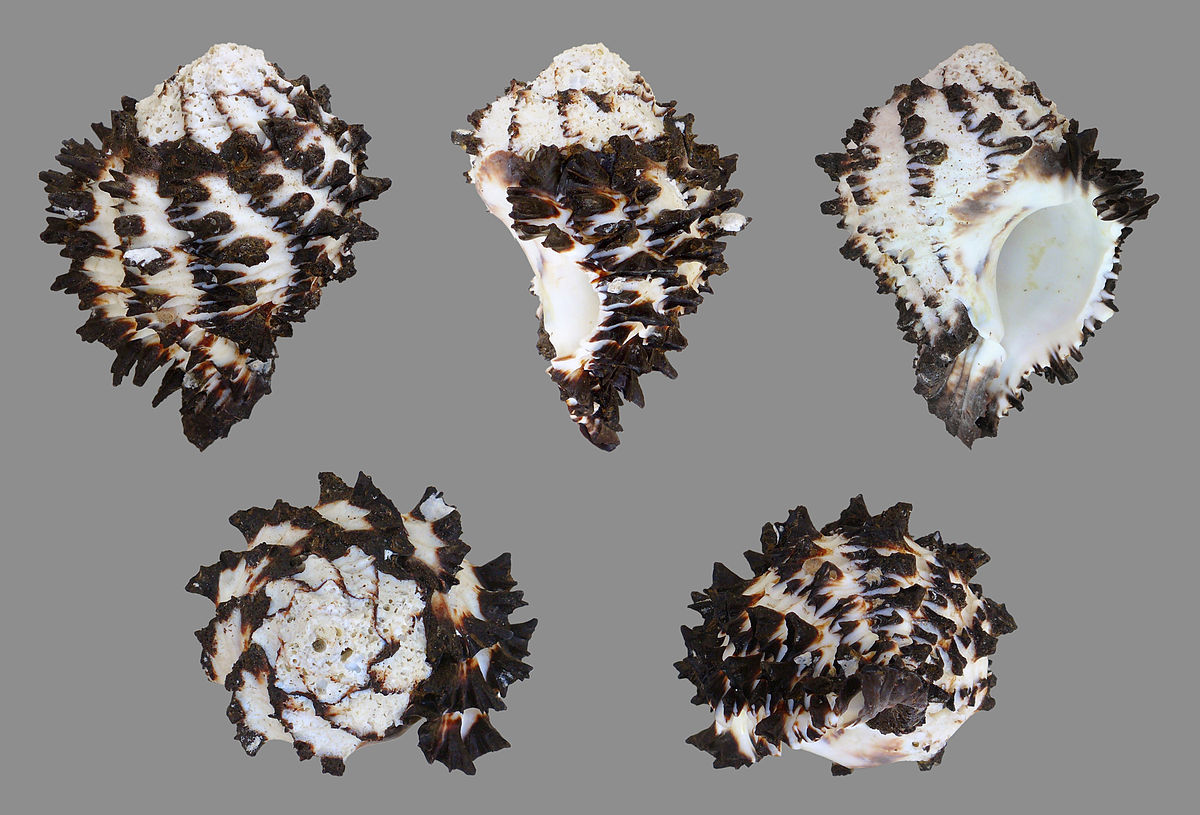
\includegraphics[scale=0.25]{./img/hexaplex_radix.jpg}
	\caption{Hexaplex radix \cite{wikipedia-hexaplex}}
	\label{fig:hexaplex-radix} % Unique label used for referencing the figure in-text
	%\addcontentsline{toc}{figure}{Figure \ref{fig:placeholder}} % Uncomment to add the figure to the table of contents
\end{figure}

The main objective would be to create a model that closely resembles the shell and to 3D print it. After completing the main objective it may be possible to generalize the methods used to describe various other shells.

\section*{Ideas for How to Approach}

A parametric surface of the main spiral pattern of hexaplex radix can be made by using a generating curve using previously known techniques, such as parametric log spirals \cite{abss}, or generalized cylinders \cite{VANDERHELM1998505}.

The pigmentation pattern can likely be generated using known RD techniques.

The shape of the protrusions suggest that they can be produced by some kind of fractal surface. Two possible methods to generate them on the model would be to: create an initial displacement map using RD then apply a noise-based multifractal at the local area, or to use RD to find the locations of the protrusion then use CSG to add the fractal surfaces to the locations. Likely much of the project will deal with this problem.

If those techniques work then they may be applied in the modeling of other intricate shells such as:

\begin{figure}[h]
	\centering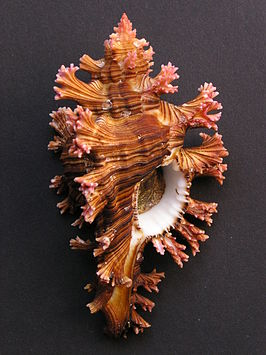
\includegraphics[scale=0.7]{./img/chicoreus_palmarosae.jpg}
	\caption{Chicoreus palmarosae \cite{wikipedia-chicoreus}}
	\label{fig:chicoreus_palmarosae} % Unique label used for referencing the figure in-text
	%\addcontentsline{toc}{figure}{Figure \ref{fig:placeholder}} % Uncomment to add the figure to the table of contents
\end{figure}

The above shell has protrusions that have coral-like structure, which has been studied using fractal modeling by Kaandorp \cite{fmgfb}.

\section*{Tools}

Comité has used Java and ImageJ for RD texture generation and Python with Blender to produce models that can be 3D printed \cite{3dprinting-seashells}. It seems like a reasonable idea to have the same setup, but I may test other tools in the preliminary weeks to see their capabilities. As far as I know for texture generation there exist image processing libraries for most popular language. For 3D modeling with CSG it may be easier to use a ray tracer, such as POV-Ray, in combination with a modeler. The benefits of CAD software are also unclear to me, so I think I may experiment with tools like OpenSCAD.

3D printed prototypes can be cheaply produced at the Carleton Library or the Nepean-Centerpointe Library. For a final product, online services such as Shapeways have higher quality printers and materials that can produce the level of texture detail necessary to make a lifelike model.

\section*{Deliverables}

\begin{enumerate}
	\item{
		Source code used to generate texture and models.
	}
	\item{
		The models and textures of hexaplex radix, as well as any other shells produced.
	}
	\item{
		3D printed versions of the models produced.
	}
	\item{
		Final report.
	}
\end{enumerate}

\section*{Biweekly Timeline}

\begin{center}
	\begin{tabular}{ | l | p{130mm} | }
		\hline
		Start Date & Task \\ \hline
		Jan. 21 & Experiment with tools. Try to create some RD textures and simple shell models that can be printed. Research CSG and fractal modeling techniques. \\ \hline
		
		Feb. 4 & Create a simple shell model for hexaplex radix. Try to create an appropriate texture and displacement map. Try to decide on an approach to the protrusions. \\ \hline
		
		Feb. 18 & Continue trying to create aspects of the model. Attempt to create the protrusions on the shell. 
		
		\textbf{Mar. 1 Give mid-term report to supervisor.} \\ \hline
		
		Mar. 4 & Continue working on the modeling of the shell. Research the 3D printing. \\ \hline
		
		Mar. 18 & Finish Modeling the shell. Try to get a 3D printed version. Try applying the techniques to additional shells. \\ \hline
		
		Apr. 1 & Work on the report. Continue working on generalizing the method.
		
		 \textbf{Apr. 8 Give first draft of report to supervisor.}  \\ \hline
		
		Apr. 15 & Complete any parts that remain. Polish the report. 
		
		\textbf{Apr. 22  Submit final report.} \\ \hline
	\end{tabular}
\end{center}